%
% Cifradores de flujo sínccronos, capítulo de antecedentes.
% Proyecto Lovelace.
%

\subsection{Síncronos}

Un cifrado de flujo síncrono es aquel en el que el flujo de la llave es
generado de manera independiente del texto en claro y del texto cifrado. Se
puede definir un modelo general con las siguientes tres ecuaciones.

\begin{equation}
  \label{sinc:cambio_de_estado}
  e_{i+1} = f(e_i, L)
\end{equation}

\begin{equation}
  \label{sinc:flujo_de_llave}
  l_i = g(e_i, L)
\end{equation}

\begin{equation}
  \label{sinc:funcion_de_salida}
  c_i = h(l_i, m_i)
\end{equation}

\vspace{0.5cm}

La letra $ e $ representa el estado del cifrado,$ L $ es la llave, $ l $ es
la salida del flujo de llave, $ c $ es el texto cifrado y $ m $ es el texto en
claro. La función de la ecuación \ref{sinc:cambio_de_estado} ($ f $) es la que
describe el cambio de estado; este se determina a partir del estado actual y
de la llave. En la ecuación \ref{sinc:flujo_de_llave} se describe la acción del
flujo de llave ($ g $): para determinar el próximo símbolo se emplea solamente
el estado actual y la llave. La tercera ecuación (\ref{sinc:funcion_de_salida},
$ h $) describe la acción de combinar el flujo de la llave con el mensaje, y
así obtener el texto cifrado.

% TODO: referencia a sección de OFB.

En la figura \ref{flujo_sincrono} se describe de manera gráfica las operaciones
de cifrado y descifrado; estas guardan muchas similitudes con el modo de
operación OFB, con la única excepción de que este trabaja con bloques del tamaño
del cifrado subyacente. En otras palabras, si definiéramos el tamaño del bloque
(y en consecuencia el tamaño del vector de inicialización) como 1, entonces
OFB sería un cifrado de flujo síncrono.

\vspace{0.5cm}

\begin{figure}[H]
  \centering
  \begin{subfigure}{0.45\textwidth}
    \begin{center}
      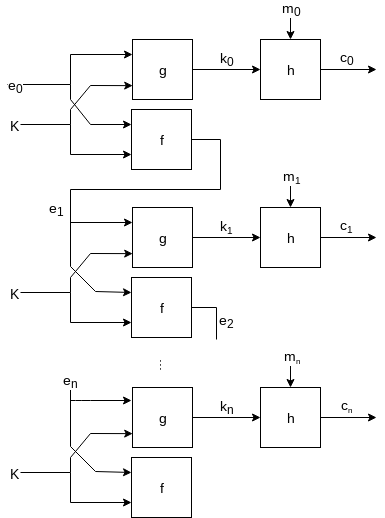
\includegraphics[width=0.9\linewidth]
        {contenidos/antecedentes/cifrados_de_flujo/diagramas/sincrono_cifrado.png}
      \caption{Cifrado.}
    \end{center}
  \end{subfigure}
  \begin{subfigure}{0.45\textwidth}
    \begin{center}
      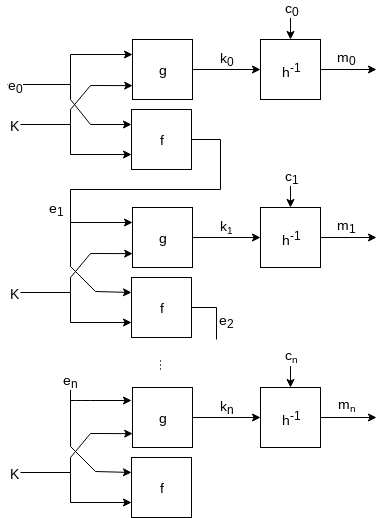
\includegraphics[width=0.9\linewidth]
        {contenidos/antecedentes/cifrados_de_flujo/diagramas/sincrono_descifrado.png}
      \caption{Descifrado.}
    \end{center}
  \end{subfigure}
  \caption{Esquema general de un cifrado de flujo síncrono.}
  \label{flujo_sincrono}
\end{figure}

El nombre de esta categoría proviene del hecho de que ambos entes del proceso
comunicativo (emisor y receptor) deben encontrarse sincronizados (usar la misma
llave y encontrarse en la misma posición) para que la comunicación tenga éxito:
si se insertan dígitos extras al mensaje cifrado, la sincronización se pierde.
Los cifrados de flujo síncronos no tienen propagación de error: aunque ciertos
bits sean modificados (pero no borrados) durante su transmisión, el resto del
mensaje sigue siendo descifrable.
